% Copyright 2004 by Till Tantau <tantau@users.sourceforge.net>.
%
% In principle, this file can be redistributed and/or modified under
% the terms of the GNU Public License, version 2.
%
% However, this file is supposed to be a template to be modified
% for your own needs. For this reason, if you use this file as a
% template and not specifically distribute it as part of a another
% package/program, I grant the extra permission to freely copy and
% modify this file as you see fit and even to delete this copyright
% notice. 

\documentclass{beamer}

% There are many different themes available for Beamer. A comprehensive
% list with examples is given here:
% http://deic.uab.es/~iblanes/beamer_gallery/index_by_theme.html
% You can uncomment the themes below if you would like to use a different
% one:
%\usetheme{AnnArbor}
%\usetheme{Antibes}
%\usetheme{Bergen}
%\usetheme{Berkeley}
%\usetheme{Berlin}
%\usetheme{Boadilla}
%\usetheme{boxes}
%\usetheme{CambridgeUS}
%\usetheme{Copenhagen}
%\usetheme{Darmstadt}
%\usetheme{default}
%\usetheme{Frankfurt}
%\usetheme{Goettingen}
%\usetheme{Hannover}
%\usetheme{Ilmenau}
%\usetheme{JuanLesPins}
%\usetheme{Luebeck}
\usetheme{Madrid}
%\usetheme{Malmoe}
%\usetheme{Marburg}
%\usetheme{Montpellier}
%\usetheme{PaloAlto}
%\usetheme{Pittsburgh}
%\usetheme{Rochester}
%\usetheme{Singapore}
%\usetheme{Szeged}
%\usetheme{Warsaw}

\usepackage{kotex}
\usepackage{braket}
\usepackage{array}
\usepackage{calc}
\usepackage{datetime}


\usepackage{listings}


\title{Lecture 3.5 : Decision Tree / SVM }

% A subtitle is optional and this may be deleted
\subtitle{Fastcampus Math Camp}

\author{신승우}
% - Give the names in the same order as the appear in the paper.
% - Use the \inst{?} command only if the authors have different
%   affiliation.

% \institute[Universities of Somewhere and Elsewhere] % (optional, but mostly needed)
% {
  % \inst{1}%
  % Department of Computer Science\\
  % University of Somewhere
  % \and
  % \inst{2}%
  % Department of Theoretical Philosophy\\
  % University of Elsewhere}
% - Use the \inst command only if there are several affiliations.
% - Keep it simple, no one is interested in your street address.

% - Either use conference name or its abbreviation.
% - Not really informative to the audience, more for people (including
%   yourself) who are reading the slides online

\subject{Theoretical Computer Science}

% This is only inserted into the PDF information catalog. Can be left
% out. 

% If you have a file called "university-logo-filename.xxx", where xxx
% is a graphic format that can be processed by latex or pdflatex,
% resp., then you can add a logo as follows:

% \pgfdeclareimage[height=0.5cm]{university-logo}{university-logo-filename}
% \logo{\pgfuseimage{university-logo}}

% Delete this, if you do not want the table of contents to pop up at
% the beginning of each subsection:


% Let's get started
\begin{document}

\begin{frame}
  \titlepage
\end{frame}

\begin{frame}{Outline}
  \tableofcontents[hideallsubsections]
  % You might wish to add the option [pausesections]
\end{frame}

% Section and subsections will appear in the presentation overview
% and table of contents.

\begin{frame}{}
\begin{itemize}{}
\item 
\end{itemize}

\end{frame}

\section{Introduction to Machine Learing} 

\subsection{Machine Learining의 개념} 



\begin{frame}[allowframebreaks]{인공지능의 발전과정}
초창기 인공지능은 
\begin{itemize} 
\item rule-based : 수많은 사람이 넣은 규칙을 이용해서 판단 
\item logical AI : 논리적인 규칙을 만들고 연역을 이용해서 판단 
\end{itemize}

하는 등, 대부분 deterministic하고 white-box 모델이였다. 이런 모델의 경우 장점이 

\begin{itemize} 
\item 얻어낸 결과를 설명 가능하며, 디버깅도 가능하다. 
\item 많은 계산양을 요구하지 않는다. 
\item 도메인 지식을 바로 적용할 수 있다. 
\end{itemize}

였으나, 인간이 명확한 규칙을 만들기 어려운 일(이미지 인식, 바둑 등)들에서는 위와 같은 인공지능을 구현하기 어려웠다. 

그래서 통계적인 방법을 이용한 Machine Learning이 대두하였다. 
\end{frame}

\begin{frame}{Machine Learning}

머신 러닝이란 통계적인 추론을 통해서 알고리즘을 학습시켜, 결과물을 얻어내는 방법이다. Mitchell의 정의가 눈여겨볼만하다. 
\begin{block}{Machine Learning}
A computer program is said to learn from experience E with respect to some class of tasks T and performance measure P, if its performance at tasks in T, as measured by P, improves with experience E
\end{block} 

\end{frame}

\begin{frame}{Machine Learning의 분류}

머신 러닝은 학습 데이터의 유무와 결과물의 종류에 따라서 분류된다. 
\begin{itemize}
\item 학습 데이터의 유무에 따른 분류
\begin{itemize} 
\item 지도학습 : 인간이 라벨을 달아준 데이터가 있는 경우. 
\item 비지도학습 : 그러한 데이터가 없는 경우 
\end{itemize}
\item 결과물의 종류에 따른 분류
\begin{itemize} 
\item 분류 : 결과물이 이산적인 라벨일 경우. 
\item 회귀 : 결과물이 연속적인 실수일 경우. 
\end{itemize}
\end{itemize}

오늘은 위 분류 중 지도학습/분류학습에 해당되는 알고리즘 2개를 살펴볼 것입니다. 

\end{frame}


\begin{frame}{Basic Assumption}

오늘 배우는 알고리즘은 의사결정나무와 svm이며, 이 두 경우에 모두 다음을 가정한다. 

\begin{itemize} 
\item 데이터 D는 각 데이터의 feature $\vec{x}_i$와 라벨 $y_i$로 구성된다. 오늘은 라벨이 0 혹은 1인 경우만 다룰 것이다. 
\item 학습의 목적은 새로운 데이터 $\vec{z}$ 가 들어왓을 때, 적절한 라벨을 골라 주는 것이다. 이를 위해서 데이터를 test와 train 두 개의 셋으로 나눈다. 
\end{itemize}

각 데이터마다 feature이 n개가 있다고 할 때, 데이터 각각은 n차원 공간의 점 하나로 볼 수 있다. 이 때 오늘 우리가 다룰 것은 결국 n차원 공간에서 두 가지 유형의 점을 잘 나누는 평면을 찾는 것으로 볼 수 있다. 곡면의 경우는 추후 다룰 것이다. 
\end{frame}



\subsection{Decision Tree} 

\begin{frame}{Decision Tree}
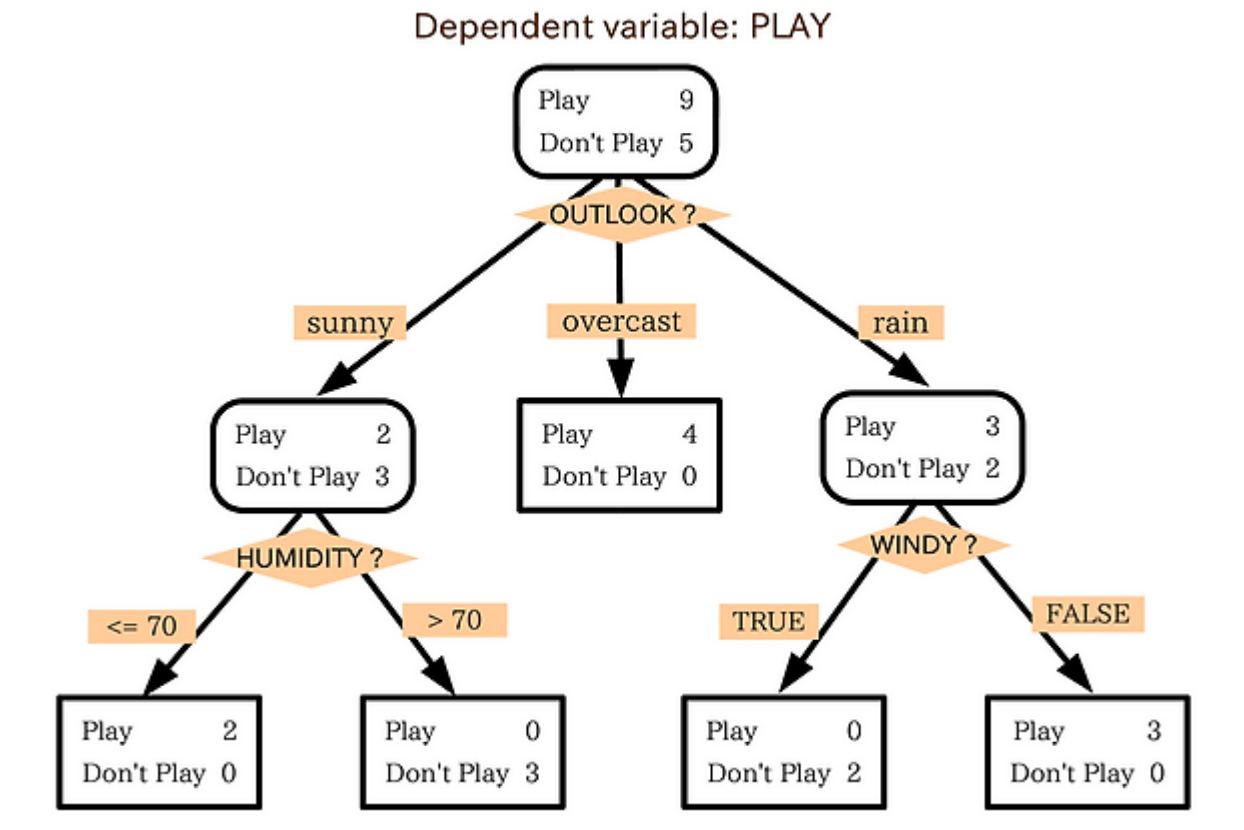
\includegraphics[width=5cm,keepaspectratio]{decisiontree}

의사결정나무는 트리의 일종으로, leaf node가 아닌 노드에는 predicate를 가지고 있고 leaf node에는 결과 라벨을 담고 있다. 의사결정나무를 이용한 결정은 root에서 시작해서, 각 노드들의 predicate를 거치는 것으로 결정된다. 
\end{frame}



\begin{frame}{Decision Tree} 
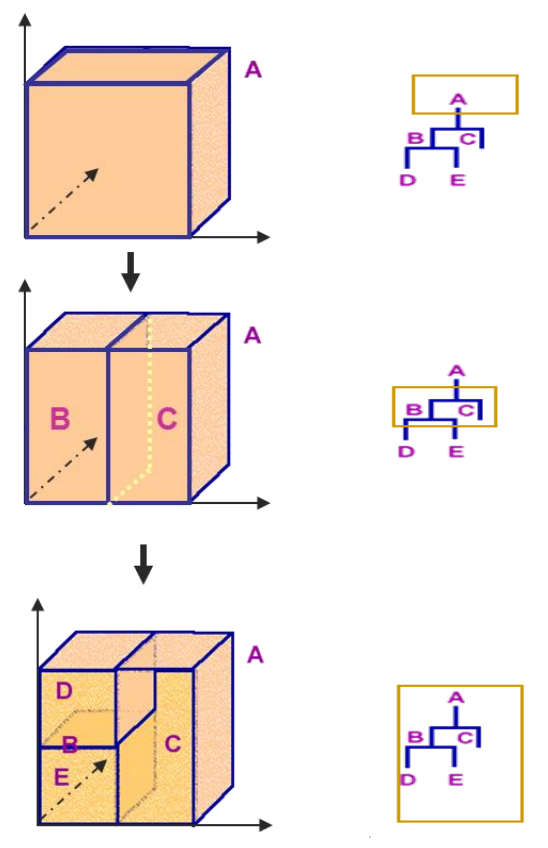
\includegraphics[height=8cm,keepaspectratio]{space}
\end{frame}

\begin{frame}{Training Decision Tree}

의사결정나무를 학습시키는 것은 주어진 데이터 상에서 가장 적절한 predicate들을 추출하는 것이다. 여기서 \textbf{적절함}이란, 가장 많은 정보를 얻을 수 있는 기준을 말한다. 그 기준을 information gain이라 하며, 엔트로피의 차이로 정한다. 
\end{frame}

\begin{frame}{What is Entropy?}
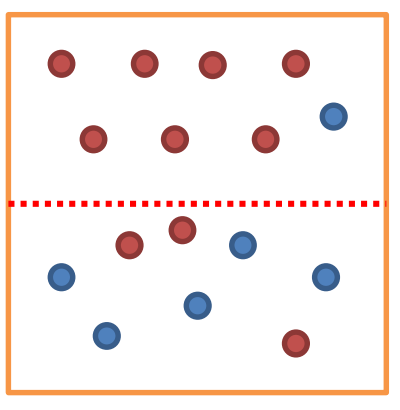
\includegraphics[height=8cm,keepaspectratio]{entropy}

\end{frame}

\begin{frame} 

엔트로피는 물리학에서 나온 개념으로, 어떤 계의 혼잡한 정도를 나타내는 개념이며 $p_i log (p_i)$로 정의된다. 예를 들어서 위 계에서, 분할 전과 분할 후의 엔트로피를 계산해 보자. \\
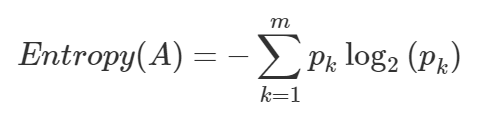
\includegraphics[height=1cm,keepaspectratio]{ent0} \\
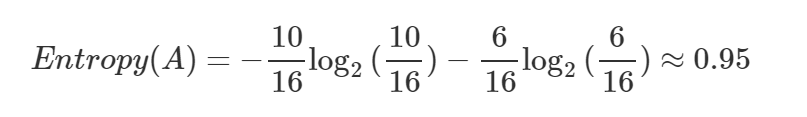
\includegraphics[height=1cm,keepaspectratio]{ent1}\\
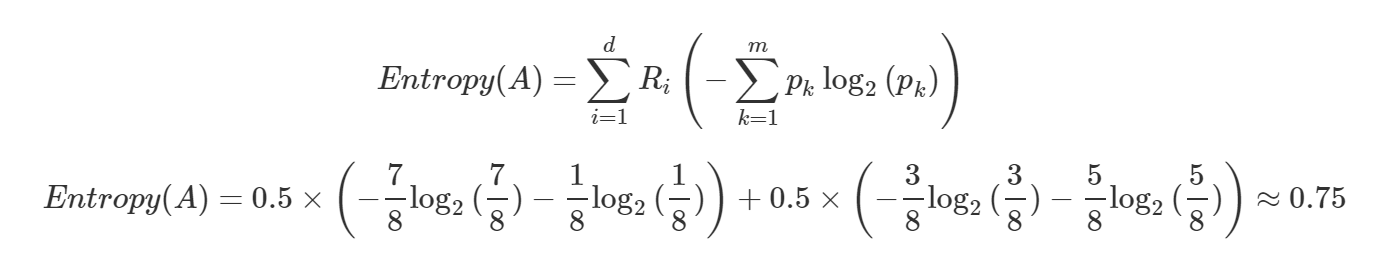
\includegraphics[height=2cm,keepaspectratio]{ent2}\\

이 때, 이 엔트로피의 차이를 information gain이라고 정의하고, information gain을 최대화하는 threshold를 찾는 것을 목표로 한다. 
\end{frame}

\begin{frame}{적절한 threshold의 탐색}

다음과 같은 방법으로 threshold를 탐색한다. 

\begin{itemize} 
\item 각 feature을 기준으로 모든 데이터를 정렬한다. 
\item 정렬된 데이터를 기준으로, 각 데이터의 feature을 threshold를 기준으로 information gain을 계산한다. 
\item 최대값을 주는 feature을 리턴한다. 
\end{itemize}

\end{frame}


\begin{frame}{Decision Tree의 학습} 

위와 같이 threshold를 탐색하는 방식을 재귀적으로 적용한다. 알고리즘은 다음과 같다. 

\begin{itemize} 
\item feature들 중 하나를 고른다. 
\item 위와 같은 방법으로 고른 feature에 대한 threshold를 기준으로 데이터셋을 나눈다. 
\begin{itemize} 
\item 트리의 노드에 고른 feature과 threshold를 저장한다. 
\item 나눠진 데이터셋에 대해서 각자 feature을 골라서, 위 과정을 반복한다. 
\end{itemize}
\item 모든 feature을 다 쓰면 학습을 종료한다. 
\end{itemize}

\end{frame}

\begin{frame} {Code Review/Evaluation} 
중고차 거래 데이터를 decision tree를 이용하여 분류해보자. decision tree 폴더 안에 data/에 있는 데이터를 이용하여, 주어진 차에 대한 데이터를 기반으로 중고차의 상태를 예측하는 의사결정나무를 학습시킨다. 
\end{frame}


\subsection{Support Vector Machine} 


\begin{frame}{Support Vector Machine}
SVM은 위 의사결정트리 알고리즘과 사실상 거의 같다. 다만 다른 점은, 꼭 축에 수직한 평면으로 나누지 않는다는 점과 필요한 경우 kernel function을 이용하여 곡면을 만든다는 점이다. 
\end{frame}

\begin{frame}{Concept of SVM}
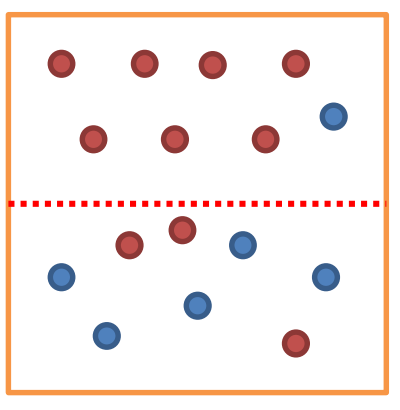
\includegraphics[height=8cm,keepaspectratio]{entropy}
\end{frame}

\begin{frame}[allowframebreaks]{Concept of SVM}
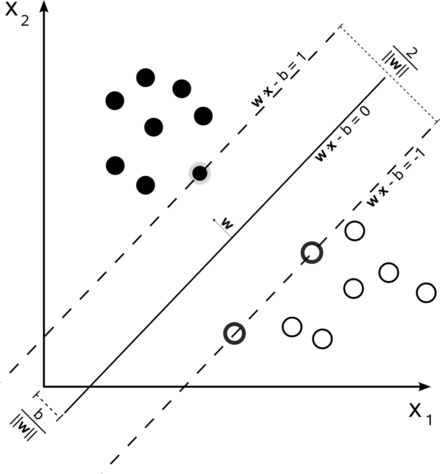
\includegraphics[height=4cm,keepaspectratio]{svmconcpet}


데이터셋 $\{(\vec{x}_i, y_i)| i = 1,2,...,n\}$에 대해서, $y_i$를 잘 분리하는 평면을 찾기 위해서는 $\vec{w} \bullet \vec{x} - \vec{b} = 0$인 평면을 찾고자 한다. 이 때, 수식적인 편의를 위해서 $y_i$를 1 혹은 -1이라고 하자. 그러면, 앞에서 정의한 평면에 대해서 다음의 두 식이 성립하도록 normalization을 할 수 있다. 


$\vec{w} \bullet \vec{x}_i - \vec{b} > 1 , y_i = 1 $

$\vec{w} \bullet \vec{x}_i - \vec{b} < -1 , y_i = -1$


위 두 식을 합치면, $y_i(\vec{w} \bullet \vec{x}_i - \vec{b} )>1$ 이라고 볼 수 있다. 즉, 이 식을 만족하는 $\vec{w}$와 $\vec{b}$를 찾으면 된다. 

\end{frame}

\begin{frame}{Concept of SVM - nonlinear case }
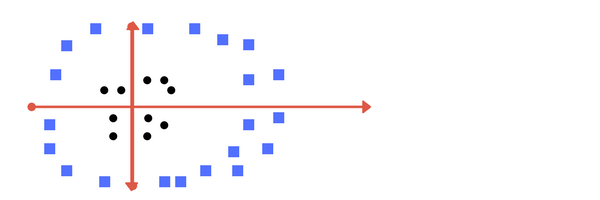
\includegraphics[height=4cm,keepaspectratio]{nonlinear}
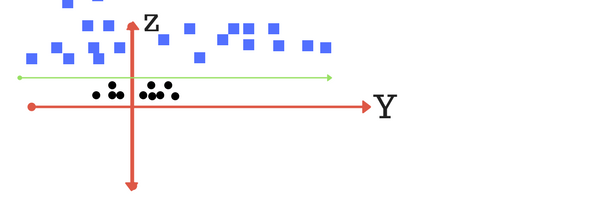
\includegraphics[height=4cm,keepaspectratio]{linear}
\end{frame}




\end{document}


